\documentclass[11pt]{article}
\textwidth 15cm 
\textheight 21.3cm
\evensidemargin -7mm
\oddsidemargin -7mm
\topmargin -1.1cm
\setlength{\parskip}{1.5ex}
\usepackage{amsfonts,amsmath,amssymb,amsthm,graphicx,systeme}
\usepackage[utf8]{inputenc}
\usepackage[english]{babel}
\usepackage{xcolor,soul}
\usepackage{tikz}
\usepackage{aeguill}
\graphicspath{ {D:/UW courses/2A/CS 246/cs246Assignment/Game_of_Constructor/final project documentation/ddl 1/} }
\renewcommand{\qedsymbol}{\rule{0.7em}{0.7em}}
\begin{document}
\parindent=0pt

\newcommand{\colorP}[1]{\colorbox{pink}{#1}}
\newcommand{\colorY}[1]{\colorbox{yellow}{#1}}
\newcommand{\Strategy}{\underline{Strategy} }
\newcommand{\Template}{\underline{Template} }
\newcommand{\Decorator}{\underline{Decorator} }

\section*{UML Diagram:}
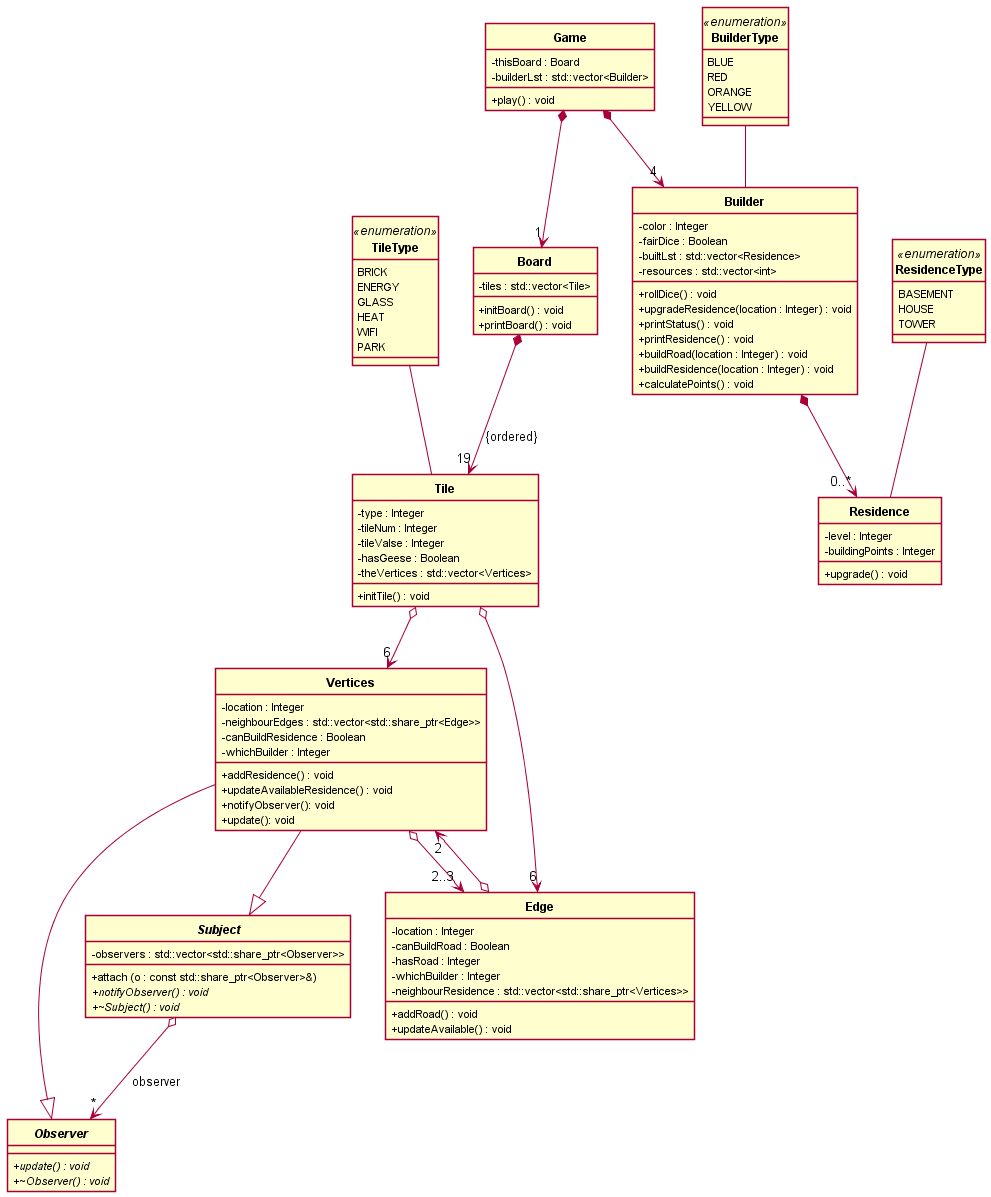
\includegraphics[width=18cm, height=20cm]{D:/UW courses/2A/CS 246/cs246Assignment/Game_of_Constructor/final project documentation/ddl 1/uml.png}

\pagebreak

\section*{Plan and Documentation Tasks:}
\begin{tabular}{|c|c|c|c|}\hline
Item & Hard Deadline & Estimated Completion time & Note \\\hline
UML Diagram - ddl \#1 & July 28, 5:00 PM & July 26, 11:59 AM & Sumbit \textbf{uml.pdf}\\\hline
Plan of attack - ddl \#1 & July 28, 5:00 PM & July 27, 11:58 AM & Sumbit \textbf{plan.pdf}\\\hline
Finalize - ddl \#1 files& July 28, 5:00 PM & July 27, 11:59 AM &\\\hline
Demo Plan - ddl \#2 & August 13, 11:59 PM & August 11, 11:58 AM & Sumbit \textbf{demo.pdf} \\
&&&in the file with project\\\hline
UML Diagram - ddl \#2 & August 13, 11:59 PM & August 11, 11:59 AM & Sumbit \textbf{uml-final.pdf}\\\hline
Design-ddl\#2 & August 13, 11:59 PM & August 12, 11:58 AM & Sumbit \textbf{design.pdf}\\\hline
Finalize-ddl\# 2 files & August 13, 11:59 PM & August 12, 11:59 AM & \\\hline
\end{tabular}

\section*{Implementation Plan:}
The following deadline will be displayed in China Time Zone, we labeled tasks with priority (\colorP{red - high}, \colorY{yellow - medium}, no label - normal) and we use the bold text represents the class we need to implement.\\
\begin{tabular}{|cc|cc|cc|}\hline
Deadline &(All at 11:59 PM) && Yifan && Jiaqi \\\hline
Monday & July 26 & $\square$ &UML Diagram-ddl \#1 & $\square$& Plan of Attack \\\hline
Tuesday & July 27 & $\square$& Finalize-ddl \#1 files & $\square$& Finalize-ddl \#1 files \\\hline
Wednesday & July 28 & $\square$ &header: \textbf{Game,Board,} & $\square$& header: \textbf{Vertices, Observer,} \\
&&& \textbf{Edge,Tile,Residence,} &&\textbf{Builder, BuilderType,} \\
&&& \textbf{ResidenceType} && \textbf{Subject,TileType}\\\hline
Thursday&July 29&$\square$ &\textbf{\colorY{Tile}}& $\square$&\textbf{Builder}\\\hline
Friday&July 30&$\square$ &\textbf{Edge}& $\square$&\textbf{\colorY{Subject}}\\\hline
Monday&August 2&$\square$ &\textbf{Board}& $\square$&\textbf{\colorY{Observer}}\\\hline
Tuesday&August 3&$\square$ &\textbf{Game}& $\square$&\textbf{Builder} Revisit\\\hline
Wednesday&August 4&$\square$ &\textbf{\colorY{Residence}}& $\square$&\textbf{\colorP{Vertices}}\\\hline
Thursday&August 5&$\square$ &\colorP{Merge \textbf{Edge} and \textbf{Vertices}}& $\square$&Merge \textbf{Subject} and \textbf{Observer}\\\hline
Friday&August 6&$\square$ &\colorY{Merge all codes and basic test}& $\square$&\colorY{Merge all codes and basic test}\\\hline
Monday&August 9&$\square$ &Extra features& $\square$&Extra features\\\hline
Tuesday&August 10&$\square$ &Extra features& $\square$&Extra features\\\hline
Wednesday&August 11&$\square$ &Final Test, UML Diagram,& $\square$&Final Test, overview,design, \\
&&& Resilience to Change&&Resilience to Change, \\
&&&&&Answer Questions\\\hline
Thursday&August 12&$\square$ &Final Test, (conclusion)&$\square$ & Final Test, (introduction)\\\hline
Friday&August 13&$\square$ &Finalize and Submit &$\square$ &Finalize and Submit\\\hline
\end{tabular}

\pagebreak
\textbf{\underline{Question 1:} You have to implement the ability to choose between randomly setting up the resources of the board and reading the resources used from a file at runtime. What design pattern could you use to implement this feature? Did you use this design pattern? Why or why not?}\\

We can use the \Strategy design pattern to implement the feature of randomly setting up the resources of the board and reading the resources used from a file a runtime. The randomness of setting up the resources of the board is controlled by user inputting the flag \textbf{-random}, based on this flag, we can apply different algorithm to control the input reading method. In addition, since this is done at runtime, then we could apply \Strategy design pattern.\\

In our own implementation, we will not apply the exact \Strategy design pattern introduced in the lecture; instead, we will extend the core idea of Strategy design pattern and simplify it. Since we only have two ways of setting up the resources of the board and reading the resources used from a file at runtime, it's a binary control, and we can simply use a Boolean variable to control with two different algorithms implemented in two different functions. If in the future, we have extra features that allow us to have a third, a fourth or more algorithms to implement this feature, we will certainly consider using the \Strategy design pattern to allow us to isolate the codes, the internal data, and the dependencies of different algorithms from the rest of the implementation.\\

\textbf{\underline{Question 2:} You must be able to switch between loaded and fair dice at run-time. What design pattern could you use to implement this feature? Did you use this design pattern? Why or why not?}\\

We can use the \Strategy design pattern to implement the feature of switching dices. The use of the dice is controlled by user inputting the command \textbf{load} and \textbf{fair}, based on this command, we can apply different algorithm to operate dice rolling when use input command \textbf{roll}. In addition, since this is done at runtime, then we could apply \Strategy design pattern.

In our own implementation, we will not apply the exact \Strategy design pattern introduced in the lecture; instead, we will extend the core idea of Strategy design pattern and simplify it. Since we only have two dices when rolling, it can be considered a binary control, and we can simply use a Boolean variable to control with two different algorithms implemented in two different functions. In this way, the implementation will be much easier since we only store a Boolean and two member functions for dice rolling. If in the future, we have extra features that allow us to have a third, a fourth or more algorithms to implement the dice we want to roll, we will certainly consider using the \Strategy design pattern to allow us to isolate the codes, the internal data, and the dependencies of different algorithms from the rest of the implementation.

\textbf{\underline{Question 3:} We have defined the game of Constructor to have a specific board layout and size. Suppose we wanted to have different game modes (e.g. hexagonal tiles, a graphical display, different sized board for a different numbers of players). What design pattern would you consider using for all of these ideas?}\\

We can use the \Template design pattern to implement the feature of settling board layout and size. The display of the board can be control by defined flags (e.g. \textbf{-hexa}, \textbf{-graphical}) we can apply different algorithm to control the essential display of the game. In addition, since the commands are inputted at compile time, hence the decision of game modes is also made using at compile time, then we could apply Template design pattern.

If we want to implement board shape feature using this \Template design pattern, a \textbf{Shape} class can be helpful with child classes being \textbf{hexagonal}, \textbf{regular}, etc. We pass instantiated child class of class \textbf{Shape} as parameters to a class \textbf{File} to control the algorithm of layout and size of the board.  Similarly, if we want to implement a graphical display feature, we apply \Template design pattern using classes to control whether we use graphical display tool such as GUI to visualize the game.

\textbf{\underline{Question 6:} Suppose we wanted to add a feature to change the tiles’ production once the game has begun. For example, being able to improve a tile so that multiple types of resources can be obtained from the tile, or reduce the quantity of resources produced by the tile over time. What design pattern(s) could you use to facilitate this ability?}\\

We can use the \Decorator design pattern to implement the feature of changing the tile' production. \Decorator design pattern lets us add this feature to the tile at run-time rather than to the class as a whole. In this way, if we want multiple types of resources from a tile, we can have two child classes of the \textbf{decorator} class namely \textbf{addition} and \textbf{remove} to be layered on top of the tile for adding one more resources and removing one resource from the existing tile. Based on the change of the tile's production, we add or remove decorator classes (or "layer") from the current tile (either with or without layers covered).

\textbf{\underline{Question 7:} Did you use any exceptions in your project? If so, where did you use them and why? If not, give an example of a place
that it would make sense to use exceptions in your project and explain why you didn’t use them.}\\

We used exceptions on users' input and input files in our projects. We use exceptions in those two cases because once we encountered invalid input or invalid files we can catch these error and throw an exception and error messages in the main function to notify the user that the input is invalid. In this way, we can make sure that all input and input files that read into the actual game are valid.\\

If we consider invalid command, including the command user use in the game round and turns, for early stage, we will assume the inputs are valid as described. However, in future implementations (such as in the extra features), we can add blocks to ensure the exceptions cannot arise by prompting invalid command message and allow user to re-input command. Moreover, such idea of handling exception and potentially some errors can also be extended in checking the validness of parameter values.

 
\end{document}